\documentclass[
svgnames,
handout,
10pt,
]{beamer}

\usepackage{pgfpages}
% \pgfpagesuselayout{2 on 1}[a4paper,border shrink=5mm]
\usepackage[utf8]{inputenc}
\usepackage{tikz}
\usetikzlibrary{arrows,calc,decorations,decorations.markings,shapes,decorations.pathmorphing,patterns}
\usepackage{booktabs}
\usepackage{array}
\usepackage{graphicx}
\usepackage{polyglossia}
\setdefaultlanguage{english}
\setotherlanguage{thai}
\newfontfamily\thaifontsf[Script=Thai,Scale=1]{Laksaman}
\graphicspath{{./pictures/}}
\usepackage{multirow}
\usetheme{metropolis}
\author{Sappinandana Akamphon}
\institute{Thammasat University}

\title{Power Transmission \textthai{(การส่งกำลัง)}}
\subtitle{ME 310: Mechanical Design}
\date{}

\begin{document}
\begin{frame}
  \maketitle 
\end{frame}

\begin{frame}{What is Power?}
  \begin{itemize}
  \item Rate of energy (input or output) in [J/s] or [W]
  \end{itemize}
\end{frame}

\begin{frame}{Power Transmission in Mechanical Systems}
  \begin{itemize}
  \item Mechanical power comes in rotational form: motors, engines, turbine
  \begin{align*}
    Power &= F v = (F r) \frac{v}{r} \\
      &= T \omega
  \end{align*}
    \item Both $T$ and $\omega$ will factor into the shaft design
  \end{itemize}
\end{frame}

\section{Mechanical Power Sources}

\begin{frame}{Mechanical Power Sources}
  \begin{enumerate}
  \item Motors \\[1em]
  \item Engines \\[1em]
  \item Turbines
  \end{enumerate} 
\end{frame}

\begin{frame}{Internal Combustion Engines}
  \begin{columns}
    \begin{column}{0.5\textwidth}
      \begin{figure}[htbp]
        \centering
        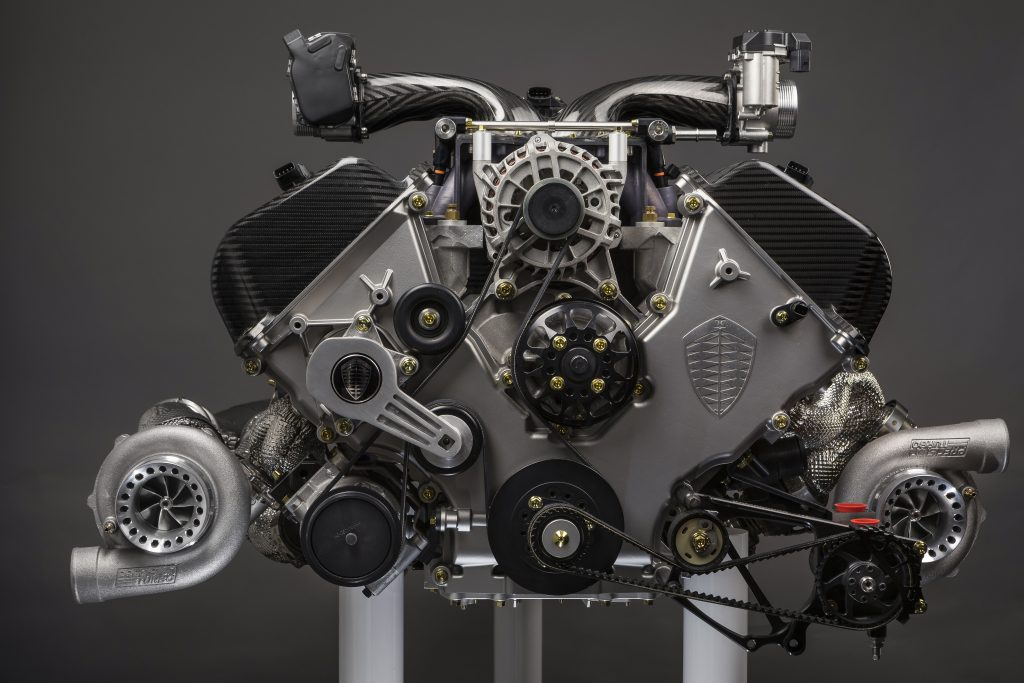
\includegraphics[width=\textwidth]{engine}
      \end{figure}
      \begin{description}
      \item[Diesel] Fuel efficiency \\
        High torque \\
        Low rpm
      \item [Gasoline] High rpm \\
        Less vibration \\
        Less weight
      \end{description}
    \end{column}
    \begin{column}{0.5\textwidth}
      \begin{figure}[htbp]
        \centering
        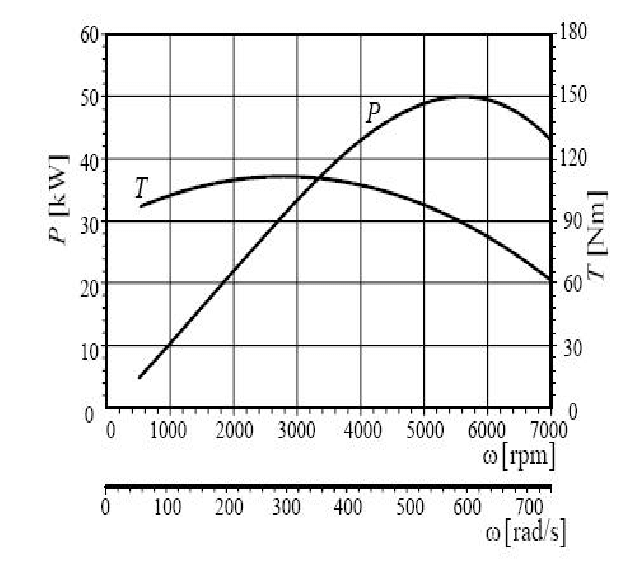
\includegraphics[width=\textwidth]{power-torque-rpm}
      \end{figure}
      \begin{description}
      \item[++] operate in remote area
      \item[- -] noise and vibration
      \item[- -] maintenance issues
      \end{description}
    \end{column}
  \end{columns}
\end{frame}

\begin{frame}{Motors}

  \centering
  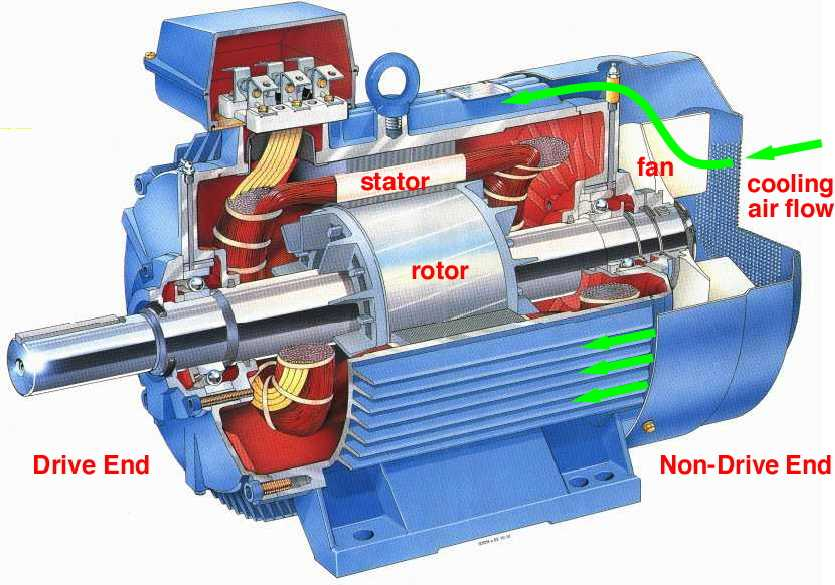
\includegraphics[height=0.6\textheight]{pictures/motor-section}

  \begin{description}
  \item[++] Smooth
  \item[++] Less noise and vibration
  \item[++] Less energy cost
  \item[- -] Need electricity
  \end{description}
  
\end{frame}

\section{Overview of Power Transmission Components}

\begin{frame}{Machine Elements for Power Transmission}
  \begin{figure}[htbp]
    \centering
    \begin{tikzpicture}[>=latex]
      \node[](auto){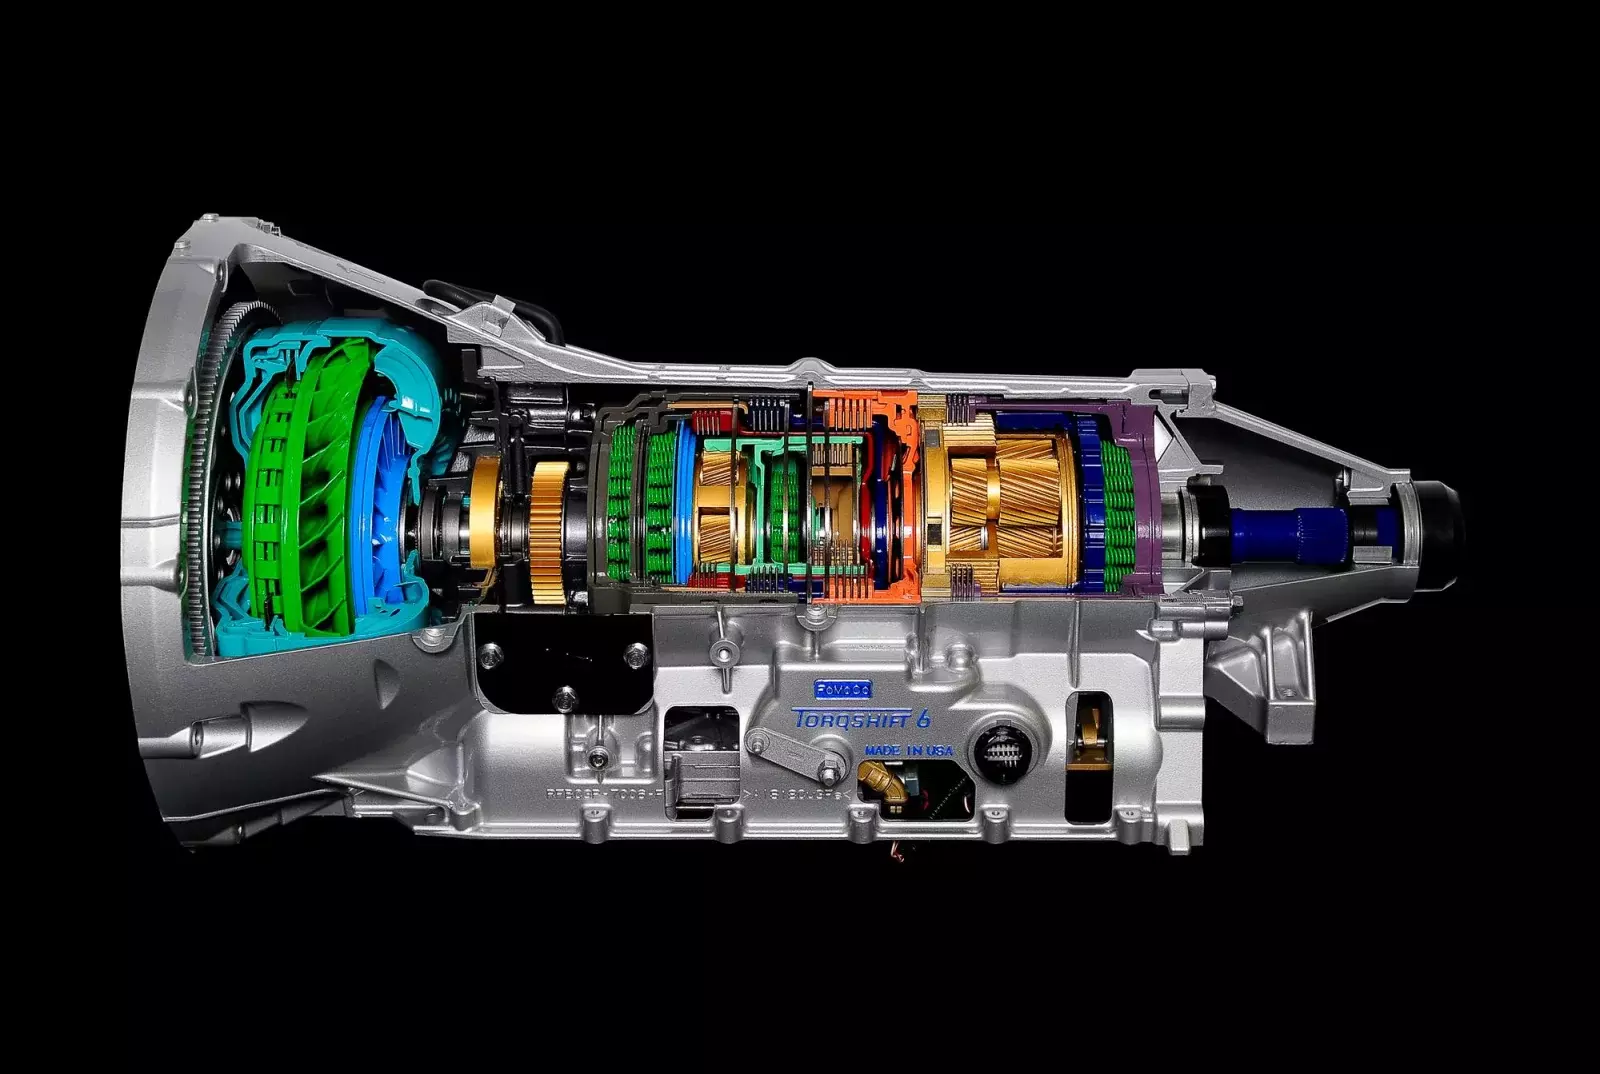
\includegraphics[width=\textwidth]{automatic-trans}};
      \draw [<-, ultra thick, White] (auto.north) ++ (-90:3) ++ (180:1) --++ (90:1) node[above]{Clutch};
      \draw [<-, ultra thick, White] (auto.north) ++ (-90:2.5) ++ (180:3) --++ (90:1) node[above]{Torque Converter (input)};
      \draw [<-, ultra thick, White] (auto.north) ++ (-90:3) ++ (0:1.3) --++ (90:1) node[above]{Planetary Gear};
      \draw [<-, ultra thick, White] (auto.north) ++ (-90:3.5) ++ (0:3) --++ (90:1) node[above]{Output Shaft};
      \draw [<-, ultra thick, White] (auto.south) ++ (90:3.5) ++ (180:1.5) --++ (-90:2) node[below]{Bearing};
      \draw [<-, ultra thick, White] (auto.south) ++ (90:3.7) ++ (0:2.5) --++ (-90:2) node[below]{Bearing};
    \end{tikzpicture}
  \end{figure}
\end{frame}

\begin{frame}{Power Transmission Drives}
  \begin{table}[htbp]
    \centering
    \begin{tabular}{ccc}
      Gear & Chain & Belt \\[2em]
      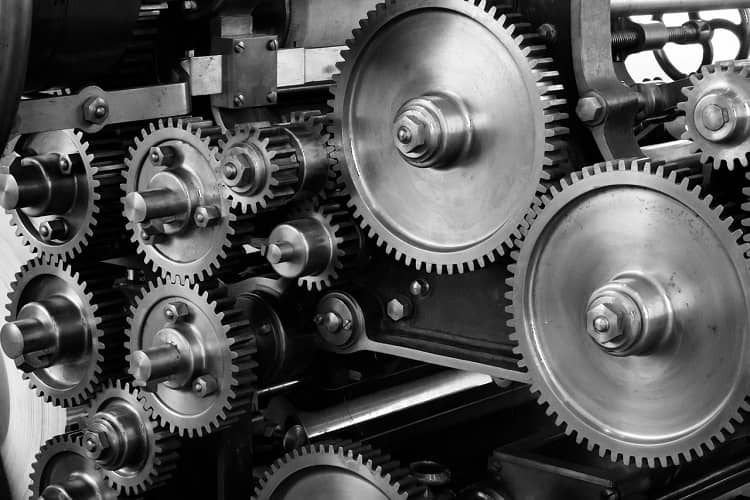
\includegraphics[width=0.3\textwidth]{gear-drive} & 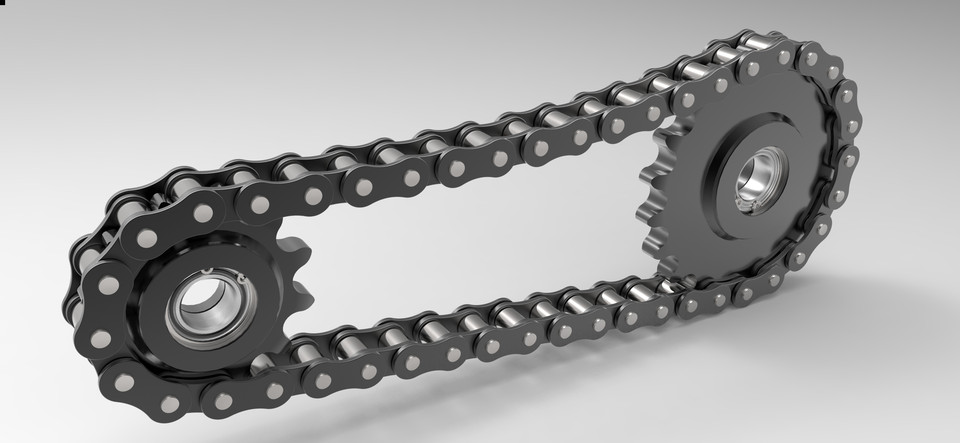
\includegraphics[width=0.3\textwidth]{chain-drive} &         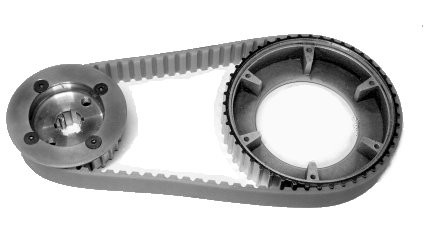
\includegraphics[width=0.3\textwidth]{belt-drive}
    \end{tabular}
  \end{table}
\end{frame}

\begin{frame}{Typical Components}
  \begin{description}
    \item[Shafts] transfer torque between aligned components over distance
    \item[Gears] transfer torque between components
    \item[Clutches] engages/disengages torque transfer
    \item[Bearings] support shaft rotation, axial, and bending loads
    \item[Pins and Keys] fix and transfer torque from components to shaft and from shaft to components
    \item[Couplings] connect two shafts with misalignment
  \end{description}
\end{frame}

\begin{frame}{Shafts}
  \begin{itemize}
    \item Most important element in power transmission system
    \item Transfer torques among all adjacent components
  \end{itemize}
  \begin{figure}[htbp]
    \centering
    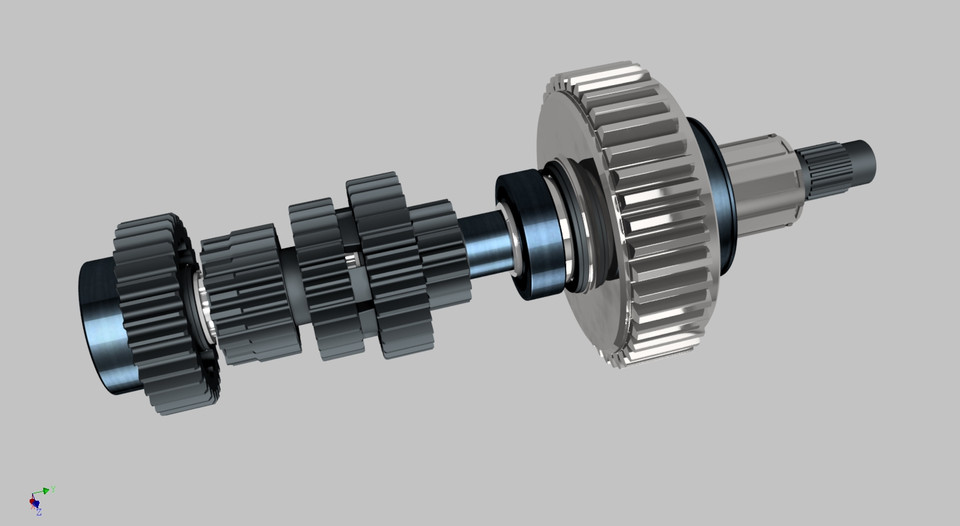
\includegraphics[width=0.8\textwidth]{shaft}
  \end{figure}
\end{frame}

\begin{frame}{Welds and Bolts}
  \begin{itemize}
    \item Shafts don't float $\rightarrow$ must be fixed somewhere
    \item Glues aren't always the answer $\rightarrow$ welds and bolts
  \end{itemize}
  \begin{figure}[htbp]
    \centering
    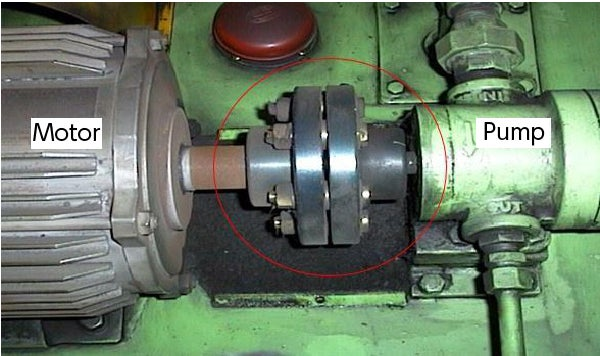
\includegraphics[width=0.8\textwidth]{shaft-bolts}
  \end{figure}
\end{frame}

\begin{frame}{Shaft Loading Conditions}
  \begin{itemize}
  \item Torque
  \item Bending $\implies$ radial load from torque transmission
  \end{itemize}
  \centering
  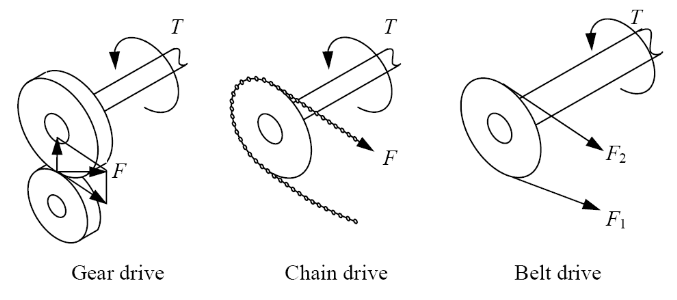
\includegraphics[width=0.8\textwidth]{pictures/torque-transmission}
  $$ F = \dfrac{T}{r \cos \theta} \hspace{1cm} F = \dfrac{T}{r} \hspace{1cm} F_1 - F_2 = \dfrac{T}{r} $$
\end{frame}

\begin{frame}{Gears vs Chain vs Belt}
  \begin{table}[htbp]
    \centering
    \begin{tabular}{lccc}
      \toprule
      Properties & Belt & Chain & Gear \\
      \midrule
      Main elements & pulleys, belt & sprockets, chain & gears \\
      \midrule
      Slip & some & none & none \\
      \midrule
      Distance & large & medium & small \\
      \midrule
      Space & large & medium & small \\
      \midrule
      Complexity & low & medium & high \\
      \midrule
      \multirow{2}{3cm}{Damage to system under Failure} & \multirow{2}{*}{none} & \multirow{2}{*}{small - medium} & \multirow{2}{*}{serious} \\
      &&& \\
      \midrule
      Life & short & medium & long \\
      \midrule
      Lubrication & not required & required & required \\
      \midrule
      Installation & easy & medium & hard \\
      \midrule
      Speed & low & medium & high \\
      \bottomrule
    \end{tabular}
  \end{table}
\end{frame}

\begin{frame}{Pin, Keys, Couplings}
  \begin{itemize}
    \item Fix components to shaft
    \item Transfer torques to and from shaft
  \end{itemize}
  \begin{figure}[htbp]
    \centering
    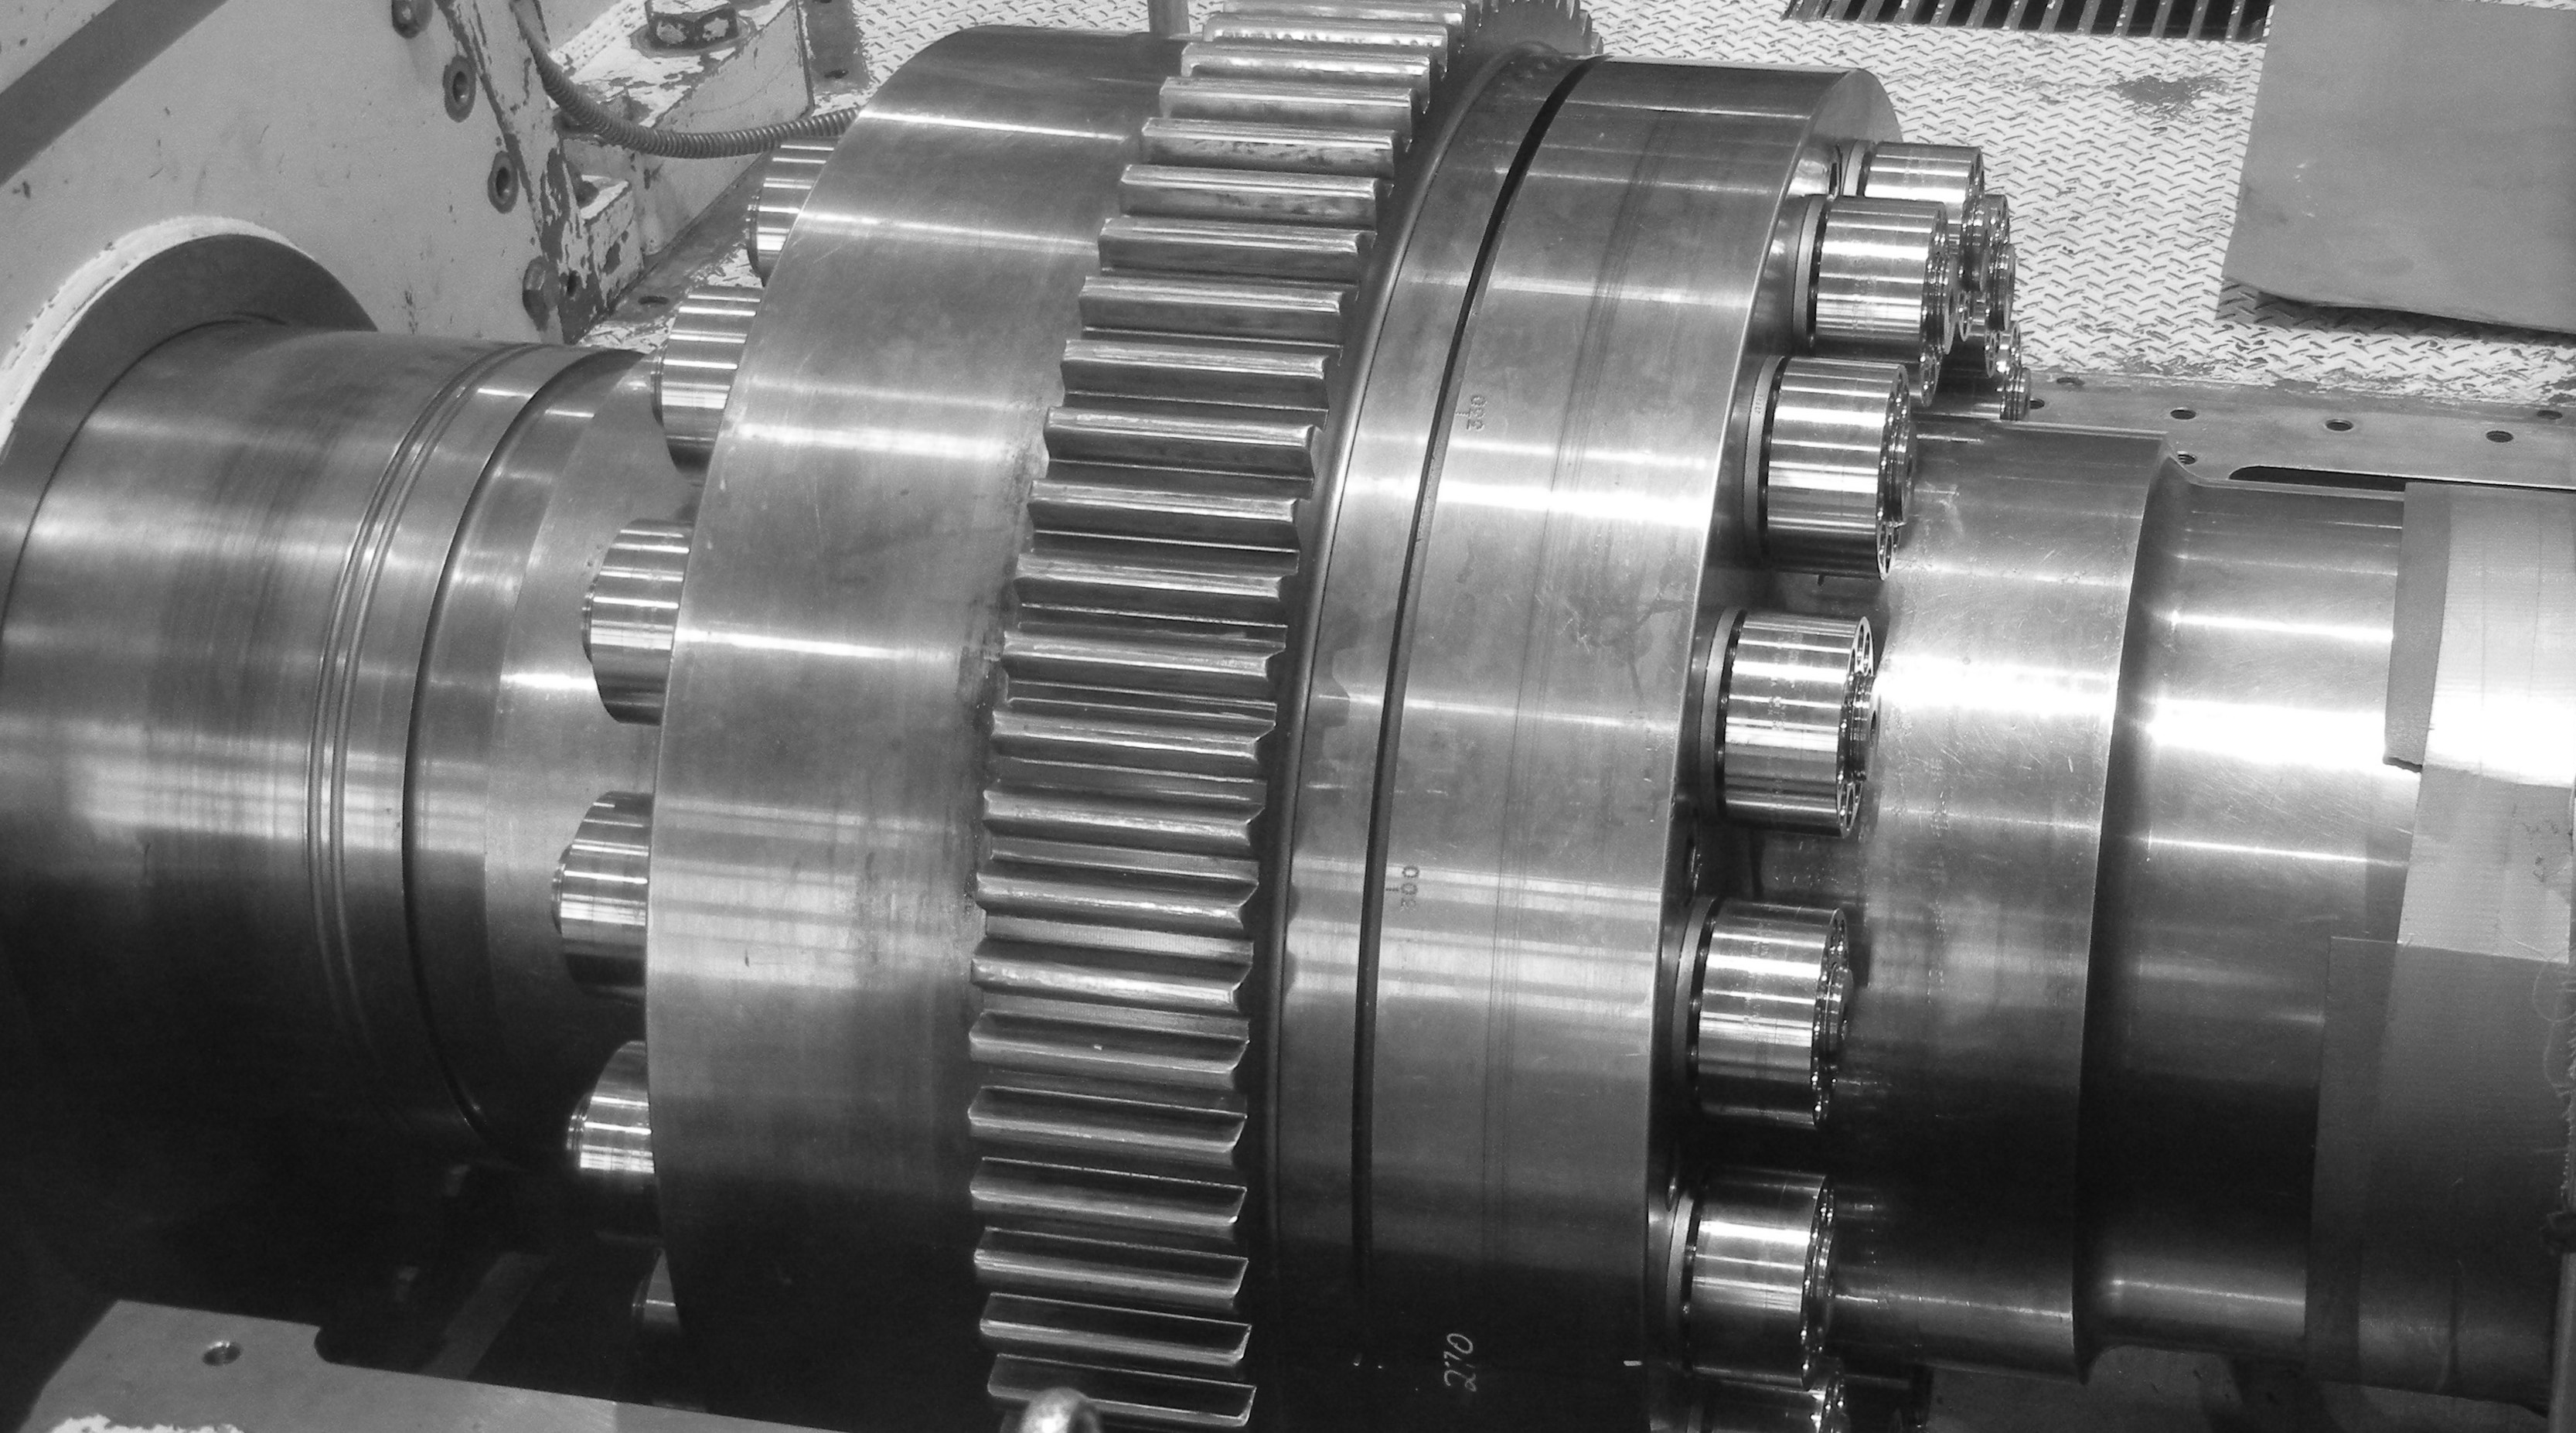
\includegraphics[width=0.8\textwidth]{turbine-coupling-bolts}
  \end{figure}
\end{frame}

\begin{frame}{Bearings}
  \begin{itemize}
    \item Support bending and axial loads from shaft
    \item Facilitate rotation
  \end{itemize}
  \begin{figure}[htbp]
    \centering
    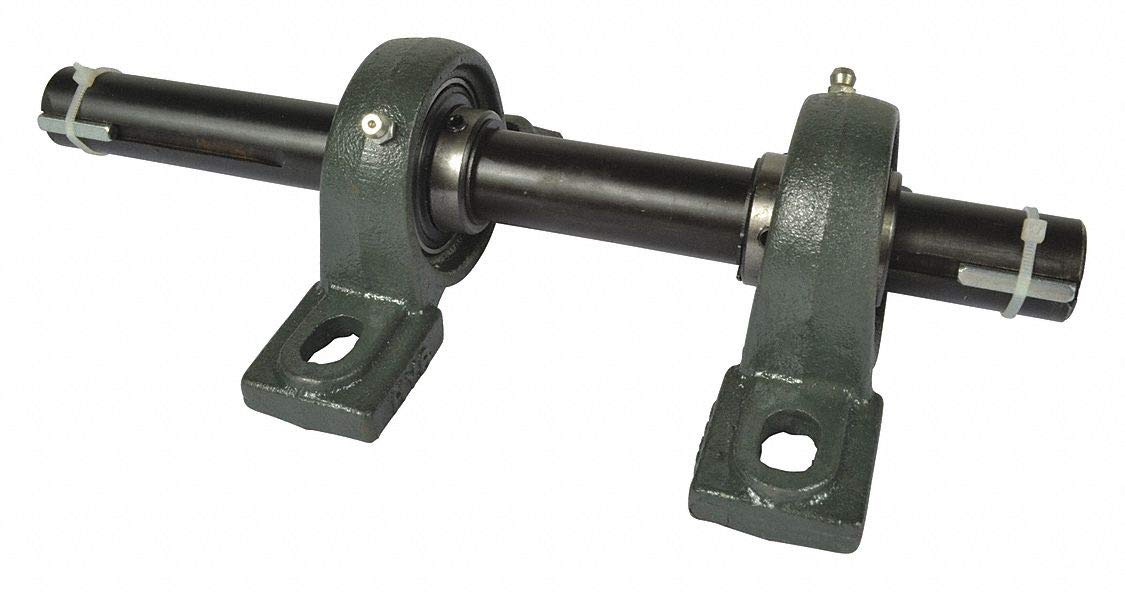
\includegraphics[width=0.8\textwidth]{bearings}
  \end{figure}
\end{frame}

\begin{frame}{Clutches and Brakes}
  \begin{itemize}
    \item Provide way to engage/disengage from drive
    \item Rely on friction or positive contact
  \end{itemize}
  \begin{figure}[htbp]
    \centering
    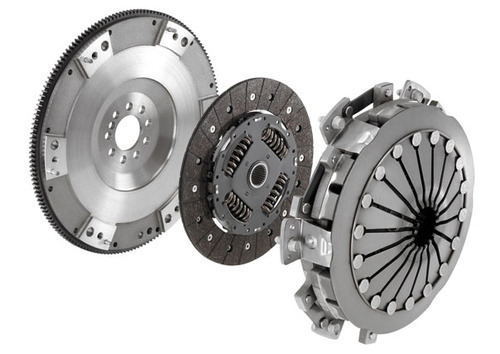
\includegraphics[width=0.7\textwidth]{clutch}
  \end{figure}
\end{frame}
\end{document}
%%% Local Variables:
%%% TeX-engine: luatex
%%% TeX-master: t
%%% End:
